\documentclass[a4paper,11pt]{report}

\usepackage{fullpage}

\usepackage{amsmath}
\usepackage{bussproofs}
\usepackage{mathpartir}
\usepackage{prooftrees}
\usepackage{color}

% Minted
\usepackage[cache=false]{minted}

\newmintinline{c}{
  fontsize=\small,
  breaklines=true
}

\newminted{c}{
  frame=single,
  framesep=2mm,
  fontsize=\scriptsize,
  mathescape
}

\newcommand*{\BBox}[1]{\draw (#1 + 0.5,0.5) -- (#1 + 1.5,0.5) -- (#1 + 1.5,-0.2)
  -- (#1 + 0.5,-0.2) -- cycle;}
\newcommand*{\SBox}[1]{}

% for finite state automata
\usepackage{tikz}
\usetikzlibrary{automata,positioning}

\author{Sylvain Julmy}
\date{\today}

\setlength{\parindent}{0pt}

\begin{document}

\begin{center}
  \Large{
    System-oriented Programming\\
    Spring 2018
  }
  
  \noindent\makebox[\linewidth]{\rule{\linewidth}{0.4pt}}
  S02
  \noindent\makebox[\linewidth]{\rule{\linewidth}{0.4pt}}

  \begin{flushleft}
    Professor : Philippe Cudré-Mauroux

    Assistant : Michael Luggen
  \end{flushleft}
  
  \noindent\makebox[\linewidth]{\rule{\linewidth}{0.4pt}}

  Submitted by Sylvain Julmy
  
  \noindent\makebox[\linewidth]{\rule{\textwidth}{1pt}}
\end{center}

\section*{Exercice 4}

\begin{itemize}
\item \verb+./wcount+
  
  This command would just invoke the program \verb+./wcount+, which would read
  the standard input (keyboard) in order to obtain something to process. We just
  have to type something, including <ENTER> char and then we send the EOF char
  by <CTRL+D>. The ouput is printed on the standard output.
  
\item \verb+./wcount < wcount.c+

  This command invoke the program \verb+./wcount+, but this time the standard
  input of the program is the file named \verb+wcount+. The ouput is printed
  on the standard output.
  
\item \verb+./wcount < wcount > test+

  This command invoke the program \verb+./wcount+, but this time the standard
  input of the program is the file named \verb+wcount.c+. The ouput is
  redirected to a file named \verb+test+.
  
\item \verb+cat wcount.c | ./wcount+

  The \verb+cat+ command will print the content of the file \verb+wcount.c+ on
  the standard output, but using the \verb+|+ operator, the standard output is
  redirected into the standard input of the \verb+./wcount+ program.
  
\item \verb+grep { wcount.c+

    The \verb+grep+ program would filter and print the content of the file
    \verb+wcount.c+. This command would print all the line of \verb+wcount.c+
    that contains a \verb+{+ symbol.
    
\item \verb+grep { wcount.c | ./wcount+

    It is the same as before except that the standard output of the \verb+grep+
    command is redirected to the standard input of the \verb+./wcount+ command.
    So the whole command would count the number of word, letter, ... of all the
    line of \verb+wcount.c+ that contains a \verb+{+ symbol.
    
\item \verb+grep -l { * | ./wcount+

    The \verb+-l+ option of \verb+grep+ is suppressing the normal output of the
    command and instead print the name of all the file from which the output
    would normally be printed. The \verb+*+ symbol represent all the file of the
    current directory. So the \verb+grep+ command would output all the filename
    of the current directory that contains the \verb+{+ symbol.
    
\end{itemize}

\section*{Exercice 5}

\begin{itemize}
\item \cinline|printf("%c %i\n", c, c);|

  We don't need any type casting here, \cinline+c+ is a variable of type
  \cinline|char| which is automaticaly seen as an integer when using the
  \verb+%i+ formatter. $65$ is the ascii value of ``A''.

  \paragraph{Output : } \verb+A 65+
  
\item \cinline|printf("%c %i\n", i, i);|

  We don't need any type casting here, \cinline+i+ is a variable of type
  \cinline+int+ which is automaticaly downgraded into a \cinline+char+ by simply
  ``cutting'' the extra-part of the \cinline+integer+ and put it into a
  \cinline+char+.
  
  \paragraph{Output : } \verb+A 65+
  
\item \cinline|printf("%f %i\n", pi, (int)pi);|

  This time we need an explicit type casting from a \cinline+float+ into an
  \cinline+integer+ because the representation, in memory, of floating point
  number and integer number is different and the compiler has to to some
  additionnal work in order to correctly transform the float value (by rounding
  the value from $3.14$ to $3$) into an integer. Without the explicit type
  casting, the number would have been read directly (the significand, the base
  and the exponant would'nt have been read separetely).
  
  \paragraph{Output : } \verb+3.140000 3+

\end{itemize}

\section*{Exercice 6}

First, the decimal value of the ascii character \verb+@+ is $64$. The output of
the program is the following

\begin{verbatim}
  @ 64 100 40
  @ 64 100 40
  @ 64 100 40
\end{verbatim}

Three times the line printed is the same because :

\begin{itemize}
\item the decimal value of \verb+@+ is 64,
\item the decimal value of \verb+\100+ is 64,
\item the decimal value of \verb+\x40+ is 64.
\end{itemize}

\section*{Exercice 7}

The output of the program is the following :

\begin{verbatim}
  1 0
  0 1 2
\end{verbatim}

In C, each enum fields is represented by an integer value from $0$ to $n-1$
where $n$ is the number of fields in the enum. Then, \verb+TRUE+ as the value
$1$ and \verb+FALSE+ as the value $0$, that's why the first line is \verb+1 0+.

For the second line, $C_1$ is initialize to \verb+RED+, which is the first field
of the \verb+color_tag+ enum, so the value of \verb+RED+ is $0$. $C_2$ is
initialize to $C_1 + 1$ which is $0 + 1 = 1$. Finally $C_3$ is initialize to
\verb+BLUE+ which is the third field of the \verb+color_tag+ enum, so the value
of \verb+BLUE+ is $3$. Then outputing $C_1$, $C_2$ and $C_3$ would be \verb+0 1 2+.

\section*{Exercice 8}

We denote by $n$ any integer not equal to $0$.

\subsection*{\cinline+p || !q+}

\begin{center}
  \begin{tabular}{@{ }c@{ }@{ }c | c@{ }@{ }c@{ }@{ }c@{ }@{ }c@{ }@{ }c@{ }@{ }c}
    p & q &  & p & \verb+||+ & \verb+!+ & q & \\
    \hline 
    $n$ & $n$ &  & $n$ & \textcolor{red}{$1$} & $0$ & $n$ & \\
    $n$ & $0$ &  & $n$ & \textcolor{red}{$1$} & $1$ & $0$ & \\
    $0$ & $n$ &  & $0$ & \textcolor{red}{$0$} & $0$ & $n$ & \\
    $0$ & $0$ &  & $0$ & \textcolor{red}{$1$} & $1$ & $0$ & \\
  \end{tabular}
\end{center}

\subsection*{\cinline+p && (p == q)+}

\begin{center}
  \begin{tabular}{@{ }c@{ }@{ }c | c@{ }@{ }c@{ }@{ }c@{ }@{}c@{}@{ }c@{ }@{ }c@{ }@{ }c@{ }@{}c@{}@{ }c}
    p & q &  & p & \verb+&&+ & ( & p & \verb+==+ & q & ) & \\
    \hline 
    $n$ & $n$ &  & $n$ & \textcolor{red}{$1$} &  & $n$ & $1$ & $n$ &  & \\
    $n$ & $0$ &  & $n$ & \textcolor{red}{$0$} &  & $n$ & $0$ & $0$ &  & \\
    $0$ & $n$ &  & $0$ & \textcolor{red}{$0$} &  & $0$ & $0$ & $n$ &  & \\
    $0$ & $0$ &  & $0$ & \textcolor{red}{$0$} &  & $0$ & $1$ & $0$ &  & \\
  \end{tabular}
\end{center}

\subsection*{\cinline+p && (p = q) || (p = !q)+}

First we add parentheses to clearly show the order of evaluation :

\cinline+( p && (p = q) ) || (p = !q)+

\begin{center}
  \begin{tabular}{@{ }c@{ }@{ }c | c@{ }@{}c@{}@{ }c@{ }@{ }c@{ }@{}c@{}@{ }c@{ }@{ }c@{ }@{ }c@{ }@{}c@{}@{}c@{}@{ }c@{ }@{}c@{}@{ }c@{ }@{ }c@{ }@{ }c@{ }@{ }c@{ }@{}c@{}@{ }c}
    p & q &  & ( & p & \verb+&&+ & ( & p & \verb+=+ & q & ) & ) & \verb+||+ & ( & p & \verb+=+ & \verb+!+ & q & ) & \\
    \hline 
    $n$ & $n$ &  &  & $n$ & $1$ &  & $n$ & $n$ & $n$ &  &  & \textcolor{red}{$1$} &  & $n$ & $0$ & $0$ & $n$ &  & \\
    $n$ & $0$ &  &  & $n$ & $0$ &  & $n$ & $0$ & $0$ &  &  & \textcolor{red}{$1$} &  & $0$ & $1$ & $1$ & $0$ &  & \\
    $0$ & $n$ &  &  & $0$ & $0$ &  & $0$ & $n$ & $n$ &  &  & \textcolor{red}{$0$} &  & $n$ & $0$ & $0$ & $n$ &  & \\
    $0$ & $0$ &  &  & $0$ & $0$ &  & $0$ & $0$ & $0$ &  &  & \textcolor{red}{$1$} &  & $0$ & $1$ & $1$ & $0$ &  & \\
  \end{tabular}
\end{center}

Finally, we verify the answer using the C program available in listing~\ref{lst:truth_ccode}.

\begin{listing}[ht]
\centering
\begin{ccode}
#include <stdio.h>

// @expr should contains variable with identifier p and q
#define truth_table_2(expr)\
    for(int i = 1; i >= 0; i--)\
    for(int j = 1; j >= 0; j--)\
    {\
        p = i;\
        q = j;\
        printf("%i\n",expr);\
    }

void main(void)
{
    int p;
    int q;

    truth_table_2(p || !q);
    printf("+---------------------------------+\n");
    truth_table_2(p && (p == q));
    printf("+---------------------------------+\n");
    truth_table_2(p && (p = q) || (p = !q));
}
\end{ccode}
\caption[]{C macro that print the result columns of the truth table for 2 variables}
\label{lst:truth_ccode}
\end{listing}

\section*{Exercice 9}

\subsection*{a)}

The output of the code would be $2$. The ternary operator could be seen as an
expression of the following form :

\cinline+   expr_t ? expr_1 : expr_2 +

\begin{itemize}
\item \cinline+expr_t+ is an expression evaluated as a boolean expression to
  determine which of the \cinline+expr_1+ or \cinline+expr_2+ to use as an
  expression in the program.
\item \cinline+expr_1+ is the expression ``returned'' if \cinline+expr_t+ is
  evaluated to $true$ (different from $0$).
\item \cinline+expr_2+ is the expression ``returned'' if \cinline+expr_t+ is
  evaluated to $false$ (equals to $0$).
\end{itemize}

\subsection*{b)}

The ternary operator is usefull for its semantics, instead of the if/else
construction which is here to determine which statement to execute or not, the
ternary construction is an expression. Which means that we can use it inside of
another expression (as seen in Figure 5 from the exercice sheet).

Ternary operator are very usefull to express simple conditional expression like
simulating the \cinline+max(a,b)+ function. By the way, if we need to do more
complicated stuff like statement or nested if/else construction, using the
standard if/else is clearly better.

\section*{Exercice 10}

\subsection*{a)}

We use unsigned integer of $n = 8$ bits for the proof. The proof would be still
valid for any value of $n$ where $n > 1$. The case where the left most bit is
not $0$ is discussed in part \textbf{b)} below.

\paragraph{Left shift : } any integer is encoded in binary and we use a sequence
of $1$ and $0$ to encode it : $x = (x_7,x_6,x_5,x_4,x_3,x_2,x_1,x_0)$. A left
shifting of $x$, denote $left$, would transform $x$ into $x'$ :

\[
  x' = (x_6,x_5,x_4,x_3,x_2,x_1,x_0,0)
\]

In order to compute the value of $x$ and $x'$, we use the following formula :

\begin{align*}
  value(x) &= x_0 \cdot 2^0 + x_1 \cdot + 2^1 + \dots + x_7 \cdot 2^7 \\
  value(x') &= 0 + x_0 \cdot 2^1 + x_1 \cdot + 2^2 + \dots + x_6 \cdot 2^7
\end{align*}

Then we have two cases :
\begin{itemize}
\item $x_i = 0$ : if a $0$ is left shifted, then the value of $x_i$ in $x'$
  don't change.
\item $x_i = 1$ : if a $1$ is left shifted, then the value of $x_i$ in $x'$ is
  two times greater that in $x$.
\end{itemize}

Now each $1$ in $x$ are doubling the value in $x'$ so that's why a left shift
multiply the value of $x$ by $2$.

\paragraph{Example : } $x = 7$, we have $x = (0,0,0,0,0,1,1,1)$. Then we compute
$x'$ :

\[
  x' = (0,0,0,0,1,1,1,0) = 14_{10} = 2 \cdot 7
\]

\paragraph{Right shift}

It is the same as the left shift, except that there is no special case if the
left most or right most bits are $1$ or $0$.

The value of $x_i$ in $x'$ would be $x_i \cdot 2^{i-1}$, which explain the $2$
time less value.

\subsection*{b)}

Now we assume that $x$ is of the following form

\[
  x = (1,x_6,x_5,x_4,x_3,x_2,x_1,x_0)
\]

In \textbf{a)} we saw that $x_7$ is not consider in the computation of $x'$, so
the value of $_7$ is ignored when left shifting the variable on the left.

If we consider a world when left shifting a variable of $n$ bits would create a
variable of $n + 1$ bits. If the left most bit is $0$, there is no problem, but
if the left most bit is $1$, then $x'$ would have the value

\[
  value(x') = 0 + x_0 \cdot 2^{1} + x_1 \cdot 2^{2} + \dots + x_{n-2} \cdot 2^{n-1} + 2^n
\]

The value of $x'$ is increase by $2^n$ more than expected, but in arithmetic
modulus $2^n$, the value of $x'$ would be


\[
  value(x') = 0 + x_0 \cdot 2^{1} + x_1 \cdot 2^{2} + \dots + x_{n-2} \cdot
  2^{n-1} + 0
\]

because $2^n \equiv 0 \mod 2^n$.

So because of the modulus $2^n$, the left shifting of a variable where $x_{n-1}$
is $1$ is not true.

\subsection*{c)}

We use the program from listing~\ref{lst:setbit}.

\begin{listing}[ht]
\centering
\begin{ccode}
#include <assert.h>
#include <stdio.h>

unsigned long setbit(unsigned long x, int n);

#define t_setbit(x,n,r) assert(setbit((unsigned long)(x),n) == (unsigned long)(r));

void main(void)
{
    t_setbit(8,0,9)
    t_setbit(100,0,101)
    t_setbit(97,0,97)
    t_setbit(7,3,15)
}

unsigned long setbit(unsigned long x, int n)
{
    return x | (((unsigned long) 1) << n);
}
\end{ccode}
\caption{Implementation of \cinline+long setbit(unsigned long x, int n);+ that
returns $x$ with the $n$th bit set to $1$.} 
\label{lst:setbit}
\end{listing}

The implementation is quiet simple, we just create a mask with the specified bit
set to $1$ and operate a bitwise and between $x$ and the mask.

\section*{Exercice 11}

Firstable, we suppose that the function $f$ has the signature \cinline+int f()+
because if $f$ would have a number of argument greater that $0$, then the
statement $f()$ would produce an error and calling a function with too many
argument is not an error.

The execution of the code can produce different results with different compilers
because the order of evalution is not defined in C. One compiler could execute
$f()$ before $g()$ and another could do the inverse.

The problem come from side effect that $f$ and $g$ could produce if, for
example, global variable are accessed in $f$ and $g$ and they are modified, then
the result of executing one function before another is strictly depending on the
compiler.

\newpage

\section*{Exercice 12}

\subsection*{a)}

\begin{center}
  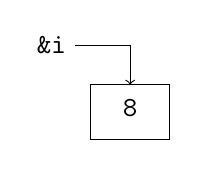
\begin{tikzpicture}[]
    \draw (0,1) node (a) {\verb|&i|};
    \draw [->] (0.3,1) -- (1,1) -- (1,0.5);
    \draw (0.5,0.5) -- (1.5,0.5) -- (1.5,-0.2) -- (0.5,-0.2) -- cycle;
    \draw (1,0.2) node (av) {\verb|8|};
  \end{tikzpicture}
  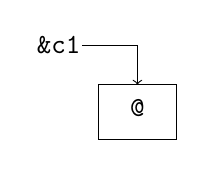
\begin{tikzpicture}[]
    \draw (0,1) node (a) {\verb|&c1|};
    \draw [->] (0.3,1) -- (1,1) -- (1,0.5);
    \BBox{0}
    \draw (1,0.2) node (av) {\verb|@|};
  \end{tikzpicture}
  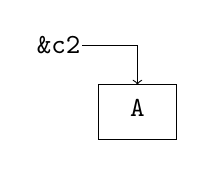
\begin{tikzpicture}[]
    \draw (0,1) node (a) {\verb|&c2|};
    \draw [->] (0.3,1) -- (1,1) -- (1,0.5);
    \BBox{0}
    \draw (1,0.2) node (av) {\verb|A|};
  \end{tikzpicture}

  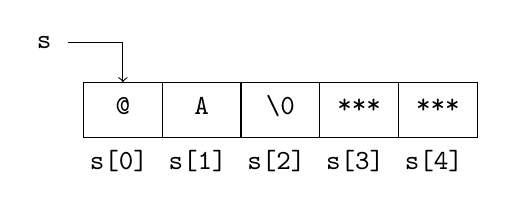
\begin{tikzpicture}[]
    \draw (0,1) node (a) {\verb|s|};
    \draw [->] (0.3,1) -- (1,1) -- (1,0.5);
    \BBox{0} \draw (0 + 0.95,-0.5) node (s0) {\verb+s[0]+};
    \BBox{1} \draw (1 + 0.95,-0.5) node (s1) {\verb+s[1]+};
    \BBox{2} \draw (2 + 0.95,-0.5) node (s2) {\verb+s[2]+};
    \BBox{3} \draw (3 + 0.95,-0.5) node (s3) {\verb+s[3]+};
    \BBox{4} \draw (4 + 0.95,-0.5) node (s4) {\verb+s[4]+};
    \draw (1,0.2) node (av) {\verb|@|};
    \draw (2,0.2) node (av) {\verb|A|};
    \draw (3,0.2) node (av) {\verb|\0|};
    \draw (4,0.2) node (av) {\verb|***|};
    \draw (5,0.2) node (av) {\verb|***|};
  \end{tikzpicture}
\end{center}

\subsection*{b)}

\begin{table}[h]
  \centering
  \begin{tabular}{ccccc}
    \multicolumn{2}{c}{Variable}                      &  & \multicolumn{2}{c}{Address} \\
    Name                    & Value                   &  & Name       & Possible value \\ \cline{2-2}
    \multicolumn{1}{c|}{i}  & \multicolumn{1}{c|}{8}  &  & \&i  & 0x00           \\ \cline{2-2}
    \multicolumn{1}{c|}{c1} & \multicolumn{1}{c|}{@}  &  & \&c1 & 0x20           \\ \cline{2-2}
    \multicolumn{1}{c|}{c2} & \multicolumn{1}{c|}{A}  &  & \&c2 & 0x40           \\ \cline{2-2}
    \multicolumn{1}{c|}{}   & \multicolumn{1}{c|}{@A} &  & s   & 0x60           \\ \cline{2-2}
  \end{tabular}
\end{table}

\subsection*{c)}

\begin{table}[h]
\centering
\begin{tabular}{lcccclccccr}
\textbf{Address}          & \multicolumn{4}{c}{\textbf{Big endian}}                                                                   &                       & \multicolumn{4}{c}{\textbf{Little endian}}                                                                & \multicolumn{1}{l}{\textbf{Address}} \\ \cline{2-5} \cline{7-10}
\multicolumn{1}{l|}{\&i}  & \multicolumn{1}{c|}{0}   & \multicolumn{1}{c|}{0}   & \multicolumn{1}{c|}{0}   & \multicolumn{1}{c|}{8}   & \multicolumn{1}{l|}{} & \multicolumn{1}{c|}{0}   & \multicolumn{1}{c|}{0}   & \multicolumn{1}{c|}{0}   & \multicolumn{1}{c|}{8}   & \&i                                  \\ \cline{2-5} \cline{7-10}
\multicolumn{1}{l|}{\&c1} & \multicolumn{1}{c|}{@}   & \multicolumn{1}{c|}{***} & \multicolumn{1}{c|}{***} & \multicolumn{1}{c|}{***} & \multicolumn{1}{l|}{} & \multicolumn{1}{c|}{***} & \multicolumn{1}{c|}{***} & \multicolumn{1}{c|}{***} & \multicolumn{1}{c|}{@}   & \&c1                                 \\ \cline{2-5} \cline{7-10}
\multicolumn{1}{l|}{\&c2} & \multicolumn{1}{c|}{A}   & \multicolumn{1}{c|}{***} & \multicolumn{1}{c|}{***} & \multicolumn{1}{c|}{***} & \multicolumn{1}{l|}{} & \multicolumn{1}{c|}{***} & \multicolumn{1}{c|}{***} & \multicolumn{1}{c|}{***} & \multicolumn{1}{c|}{A}   & \&c2                                 \\ \cline{2-5} \cline{7-10}
  \multicolumn{1}{l|}{s}    & \multicolumn{1}{c|}{@}   & \multicolumn{1}{c|}{A}   & \multicolumn{1}{c|}{$\backslash$0}  & \multicolumn{1}{c|}{***} & \multicolumn{1}{l|}{} & \multicolumn{1}{c|}{***} & \multicolumn{1}{c|}{$\backslash$0}   & \multicolumn{1}{c|}{A}   & \multicolumn{1}{c|}{@}   & s                                    \\ \cline{2-5} \cline{7-10}
\multicolumn{1}{l|}{s+4}  & \multicolumn{1}{c|}{***} & \multicolumn{1}{c|}{***} & \multicolumn{1}{c|}{***} & \multicolumn{1}{c|}{***} & \multicolumn{1}{l|}{} & \multicolumn{1}{c|}{***} & \multicolumn{1}{c|}{***} & \multicolumn{1}{c|}{***} & \multicolumn{1}{c|}{***} & s+4                                  \\ \cline{2-5} \cline{7-10}
\end{tabular}
\end{table}

\subsection*{d)}

\begin{table}[h]
\centering
\begin{tabular}{lcccclccccr}
\textbf{Address}          & \multicolumn{4}{c}{\textbf{Big endian}}                                                                     &                       & \multicolumn{4}{c}{\textbf{Little endian}}                                                                  & \multicolumn{1}{l}{\textbf{Address}} \\ \cline{2-5} \cline{7-10}
\multicolumn{1}{l|}{0x0}  & \multicolumn{1}{c|}{0}    & \multicolumn{1}{c|}{0}    & \multicolumn{1}{c|}{0}   & \multicolumn{1}{c|}{8}   & \multicolumn{1}{l|}{} & \multicolumn{1}{c|}{0}   & \multicolumn{1}{c|}{0}   & \multicolumn{1}{c|}{0}    & \multicolumn{1}{c|}{8}    & 0x0                                  \\ \cline{2-5} \cline{7-10}
\multicolumn{1}{l|}{0x4}  & \multicolumn{1}{c|}{0x40} & \multicolumn{1}{c|}{***}  & \multicolumn{1}{c|}{***} & \multicolumn{1}{c|}{***} & \multicolumn{1}{l|}{} & \multicolumn{1}{c|}{***} & \multicolumn{1}{c|}{***} & \multicolumn{1}{c|}{***}  & \multicolumn{1}{c|}{0x40} & 0x4                                  \\ \cline{2-5} \cline{7-10}
\multicolumn{1}{l|}{0x8}  & \multicolumn{1}{c|}{0x41} & \multicolumn{1}{c|}{***}  & \multicolumn{1}{c|}{***} & \multicolumn{1}{c|}{***} & \multicolumn{1}{l|}{} & \multicolumn{1}{c|}{***} & \multicolumn{1}{c|}{***} & \multicolumn{1}{c|}{***}  & \multicolumn{1}{c|}{0x41} & 0x8                                  \\ \cline{2-5} \cline{7-10}
\multicolumn{1}{l|}{0xc}  & \multicolumn{1}{c|}{0x40} & \multicolumn{1}{c|}{0x41} & \multicolumn{1}{c|}{***} & \multicolumn{1}{c|}{***} & \multicolumn{1}{l|}{} & \multicolumn{1}{c|}{***} & \multicolumn{1}{c|}{***} & \multicolumn{1}{c|}{0x41} & \multicolumn{1}{c|}{0x40} & 0xc                                  \\ \cline{2-5} \cline{7-10}
\multicolumn{1}{l|}{0x10} & \multicolumn{1}{c|}{***}  & \multicolumn{1}{c|}{***}  & \multicolumn{1}{c|}{***} & \multicolumn{1}{c|}{***} & \multicolumn{1}{l|}{} & \multicolumn{1}{c|}{***} & \multicolumn{1}{c|}{***} & \multicolumn{1}{c|}{***}  & \multicolumn{1}{c|}{***}  & 0x10                                 \\ \cline{2-5} \cline{7-10}
\end{tabular}
\end{table}

\section*{Exercice 13}

\subsection*{a)}

We use the man page of $scanf$ to figure out what is happening in the code and
specially the following two paragraphs.

\begin{verbatim}
RETURN VALUE
       On  success,  these functions return the number of input items success‐
       fully matched and assigned; this can be fewer  than  provided  for,  or
       even zero, in the event of an early matching failure.

       The  value EOF is returned if the end of input is reached before either
       the first successful conversion or a matching failure occurs.   EOF  is
       also returned if a read error occurs, in which case the error indicator
       for the stream (see ferror(3)) is set, and errno is set to indicate the
       error.
\end{verbatim}

\begin{verbatim}
The  format  string consists of a sequence of directives which describe
       how to process the sequence of input characters.  If  processing  of  a
       directive  fails,  no  further  input  is read, and scanf() returns.  A
       "failure" can be either of the following: input failure,  meaning  that
       input  characters  were  unavailable, or matching failure, meaning that
       the input was inappropriate (see below).
\end{verbatim}

The first line is correctly parsed and the values after the execution of the
first line are the following :

\begin{itemize}
\item $str =$ ``AA''
\item $i = 33$
\item $d = 2$
\end{itemize}

The second is not correctly parsed, the computer can't parse \verb+ZZ+ into an
integer and it will stop to pull characters from the standard input. So $55$ is
parsed as a string and only $1$ argument is parsed by the $scanf$ function. So
we will have the following variables and value after the second line :

\begin{itemize}
\item $str =$ ``55''
\item $i = 33$
\item $d = 1$
\end{itemize}

So ``ZZ'' remains in the standard input and that's why, when we are executing
the third line, the parsing is computed correctly and ``ZZ'' and $77$ are
correctly parsed and put into $str$ and $i$. So the variables and their value
are :

\begin{itemize}
\item $str =$ ``ZZ''
\item $i = 77$
\item $d = 2$
\end{itemize}

We note that $99$ remains in the queue of the standard input.

\subsection*{b)}

We use the following code in order to parse a character, an integer, a string
and a float.

\begin{ccode}
#include <stdio.h>
#include <assert.h>

void main(void)
{
    char c;
    int i;
    char string[10];
    float f;

    // parse the char, integer, string and the float in one line
    int res = scanf("%c %d %s %f", &c, &i, string, &f);
    assert(res == 4);

    printf("char value : %c\n"
           "integer value : %i\n"
           "string value : %s\n"
           "float value : %f\n",
           c, i, string, f);
}
\end{ccode}

We can try our code on our machine :

\begin{verbatim}
   c 123 Hello 3.4
   char value : c
   integer value : 123
   string value : Hello
   float value : 3.400000
\end{verbatim}

Which seems to correctly parse a correct input.

\end{document}
